\documentclass[CJK]{beamer}
\usepackage{CJKutf8}
\usepackage{graphicx}
\usetheme{Copenhagen}
%\usetheme{Boadilla}
\setbeamercovered{transparent}

\begin{document}
\begin{CJK*}{UTF8}{gbsn}

\title{计算机编程基础与实践}
\subtitle{---数据库基本原理与MySQL}
\author{夏永锋}
\institute[SJTU]
{上海交通大学\ 软件学院\\嵌入式实验室}

\date{\today}

\begin{frame}
	\titlepage
\end{frame}

\section*{大纲}
\begin{frame}
    \tableofcontents
\end{frame}

\begin{frame}{数据库应用的两个基本问题}
	\begin{enumerate}
		\item 如何存储?  --- 从发展轨迹来了解
		\item 如何存取?  --- 从程序与数据库的交互接口来了解
	\end{enumerate}
\end{frame}

\section{数据库发展轨迹}
\subsection{早期数据库}
\begin{frame}{早期数据库}
	\begin{block}{}
		\begin{itemize}
		\item {\bf 平面文件数据库}: 一个单一的,通常是非结构化的数据文件,比如:Word
		\item {\bf 层次数据库}:出现于20世纪60年代.基于"父/子"样式,每个父表可以拥有多个子表,但每个子表有且只有一个父表。
		\item {\bf 网状数据库}:类似于层次模型,也是基于父/子关系概念,但解除了一个子表有且只有一个父表的限制。
		\end{itemize}
	\end{block}
\end{frame}

\subsection{关系数据库}
\begin{frame}{关系数据库-表}
关系型模型是基于二维存储空间(表)的,这些表基于共有的一个字段(或一系列字段)而相互关联。
	\begin{block}{表}
		\begin{itemize}
		\item 关系数据库的基本组成单元。一个表由行和列组成(记录与字段)。
		\item 数据库中的每一个表都有一个唯一的名称(必须是唯一的完全限定名称,以模式或数据库名称作为前缀)。
		\item 表中的每一个字段都有一个唯一的名称,任何表都至少拥有一个字段,一个表的字段数限制决定于具体的实现。字段中数据必须是{\bf 同一类型}。
		\item 表中的记录并不按特定的次序来存储和检索。
		\item 好的关系设计能确保一条记录能够描述一个实体(entity)。
		\end{itemize}
	\end{block}	
\end{frame}
{\small
\begin{frame}{关系数据库-主键}
主键的任务是帮助MySQL以最快的速度把一条特定的数据记录在数据表里的位置确定下来。主键不管由单个字段还是多个字段构成,都必须满足以下条件:
	\begin{block}{}
		\begin{enumerate}
			\item 主键必须是唯一的,任意两条数据记录里的主键字段绝不允许是同样的内容
			\item 主键应该是紧凑的,理由有两条:
			\begin{itemize}
				\item {\tiny 为了加快搜索速度,主键都必须有索引,主键字段越紧凑,索引的管理工作效率越高}
				\item {\tiny 主键字段的内容几乎总是被用做另一个数据表里的外键,外键越紧凑,效率越高}
			\end{itemize}
		\end{enumerate}
		绝大多数的数据库系统上,使用32位或64位整数作为主键字段并让数据库系统为它们自动生成一组序列编号(1,2,3,...)的做法已成为一种标准化的行为,这么做的好处是{\color{blue}程序员和用户都无需再去考虑怎样才能为每一条新记录找到一个独一无二的主键值的问题}。
	\end{block}
\end{frame}
}
\begin{frame}{关系数据库-表间关系}
\begin{block}{}
{\small 对于复杂的数据,单个数据表并不能合适地表达存储,必须使用多个数据表,而且表与表之间不可能完全孤立,很多查询需要联合多个数据表。}
\end{block}
{\tiny
数据表之间的关联关系可以细分为以下3种:
\begin{itemize}
	\item 1:1关系 - 第一个数据表里的每一条数据记录分别对应着第二个数据表里的一条数据记录,同时第二个数据表里的每一条数据记录也分别对应着第一个数据表里的一条数据记录。({\color{red}不常见})
	\item 1:n关系 - 第一个数据表里的一条记录可以对应着第二个数据表中的多条记录,但反过来却不成立。({\color{red}常见})
	\item n:m关系 - 第一个数据表里的一条记录可以对应着第二个数据表里的多条记录,同时第二个数据表里的一条记录也可以对应着第一个数据表里的多条记录。({\color{red}常见})
\end{itemize}
}
\begin{block}{}
{\small 在设计数据库时,需要为每两个有着n:m关系的数据表都定义一个辅助数据表,并利用这个辅助数据表把这一组 n:m关系转化为两个1:n关系。}
\end{block}
\end{frame}
\begin{frame}{关系数据库 --- 外键}
	\begin{block}{}
	{\color{red}表间关系如何实现?}
	\end{block}
外键的任务是引用另一个数据表的某条记录,只不过这种引用关系是在构造数据库查询命令的时候而不是在声明数据表或数据列的时候定义的,如下所示:
\begin{block}{}
{\bf SELECT} titles.title, publishers.publName {\bf FROM} titles, publishers\\
{\bf WHERE} titles.publID = publishers.publID\\
{\bf ORDER BY} title
\end{block}
外键在数据表的定义声明里毫无特殊之处。在MySQL看来,外键不过是数据表里的又一普通字段。
\end{frame}

\subsection{其他类型数据库}
\begin{frame}{数据库发展轨迹 - 其他DBMS模型}
	\begin{itemize}
		\item 面向对象数据库(OODBS):直接存储对象,而不是将对象分解到文本或文本的部分字段中,然后在需要的时候将它们一起放回原处。
		\item NoSQL:主要是key/value方式存储数据,从名字就可以看出,不支持SQL。
	\end{itemize}
\end{frame}
\section{MySQL数据库设计概论}

\subsection{MySQL的特点}
\begin{frame}{MySQL的特点}
	\begin{enumerate}
		\item 关系数据库系统
		\item 客户/服务器体系:形成对照的是文件服务器系统(file-server system),如Microsoft Access, dBase和FoxPro等,不足之处-网络上运行时会因为人数的增加而变得非常缺乏效率。
		\item SQL兼容性:MySQL遵守最新的SQL标准,同时又有一些严格的限制和众多的扩展。
		\item 子查询:如SELECT * FROM table1 WHERE x IN (SELECT y from table2)
		\item 平台独立性:MySQL可以在多种平台上运行。
		\item ...
	\end{enumerate}
\end{frame}

\subsection{MySQL数据表类型}
\begin{frame}{}
	\begin{block}{}
	在创建一个新的MySQL数据表时,可以为它设置一个类型。这种做法在其他数据库系统里是不多见的。MySQL支持多种数据表类型,最重要的有:MyISAM, InnoDB。
	\end{block}
\end{frame}
\begin{frame}{MySQL数据表类型}
	\begin{block}{MyISAM}
	{\tiny
	MyISAM数据表类型的特点是成熟,稳定和易于管理。只要没有特殊理由选择其他的类型,就应该选用这个类型。
		\begin{itemize}
			\item MyISAM Static(静态MyISAM):如果数据表中的数据列各自都有预先定义好的固定长度,MySQL服务器将自动选择这种数据表类型,这种数据表的存取效率非常高,即使数据表的修改非常频繁也是如此。
			\item MyISAM Dynamic(动态MyISAM):如果在数据表的定义里有VARCHAR,xxxTEXT或xxxBLOB字段,MySQL将自动选择这种数据类型。与静态MyISAM相比,这种类型的突出特点是数据表的空间需求量往往小得多
			\item MyISAM Compressed(压缩MyISAM)
		\end{itemize}
	}
	\end{block}
	\begin{block}{InnoDB}
	{\tiny
		可以把InnoDB看做是MyISAM的一种更新换代产品,它至少增加了以下几种新功能:事务,数据行级锁定机制,外键约束条件,崩溃恢复。\\
		但InnoDB也存在一些问题缺陷:存储空间占用量等。
	}
	\end{block}	
\end{frame}
\begin{frame}{选择MyISAM还是InnoDB?}
	可以把同一数据库中的不同数据表设置为不同的类型。\\
	\begin{itemize}
		\item 如果希望以最节约空间和时间的方式来管理数据库,MyISAM数据表应该是首选;
		\item 如果应用程序需要用到事务,需要更高的安全性,或者需要允许很多用户同时修改某个数据表里的数据,InnoDB数据表就更值得考虑。
	\end{itemize}
\end{frame}
\subsection{MySQL数据类型}
\begin{frame}{}
	\begin{block}{}
		每个数据表至少会有一个数据列,而用户必须为每个数据列分别定义一个适当的数据类型!
	\end{block}
\end{frame}
\begin{frame}{MySQL数据类型-整数}
\begin{block}{}
{\tiny
在默认的情况下,INT数据类型既包括正数,也包括负数。
}
\end{block}
\centering {\tiny MySQL支持的整数数据类型}
{\tiny
\begin{tabular}{l|p{8cm}}\hline
MySQL数据类型 &  含义 \\ \hline
TINYINT(m) & 8位整数(1个字节,-128~+127);可选参数m给出的是SELECT查询结果中的数据列宽度,对取值范围没有影响。\\ \hline
SMALLINT(m) & 16位整数(2个字节,从-32768 ~ +32767)\\ \hline
MEDIUMINT(m) & 24位整数(3个字节)\\ \hline
INT(m), INTEGER(m) & 32位整数\\ \hline
BIGINT(m) & 64位整数\\ \hline
SERIAL & BIGINT AUTO\underline{\ }INCREMENT NOT NULL PRIMARY KEY的简写\\ \hline
\end{tabular}
}
{\tiny
\begin{block}{AUTO\underline{\ }INCREMENT整数}
如果给某个数据表中的一个整数数据列定义可选的AUTO\underline{\ }INCREMENT属性,那么当用户向这个数据表插入一条新记录时,MySQL就会自动地把这个整数数据列的当前最大取值加上1之后赋值给新纪录中的这个整数字段。AUTO\underline{\ }INCREMENT属性的常见用法是定义数据表的主键字段。
	\begin{itemize}
		\item 这个属性必须与NOT NULL, PRIMARY KEY或者UNIQUE属性同时使用。
		\item 每个数据表最多只能有一个AUTO\underline{\ }INCREMENT数据列。
		\item 如果AUTO\underline{\ }计数器到达了它的最大值,将不再继续递增,数据记录的插入操作也将随之无法继续进行。
	\end{itemize}
\end{block}
}
\end{frame}

\begin{frame}{MySQL数据类型-日期与时间}
\begin{center}
{\small MySQL支持的日期和时间数据类型}
\end{center}
{\tiny
\begin{tabular}{l|p{8cm}}\hline
MySQL数据类型 & 含义 \\ \hline
DATE & '2003-12-31'格式的日期值,取值范围: 1000-01-01~9999-12-31(3个字节)\\ \hline
TIME & '23:59:59'格式的时间值,取值范围: $\pm$838:59:59(3个字节)\\ \hline
DATETIME & '2003-12-31 23:59:59'格式的DATE加TIME组合\\ \hline
YEAR & 年份,取值范围:100~2155(1个字节)\\ \hline
\end{tabular}}
\end{frame}

\begin{frame}{MySQL数据类型-字符串}
\begin{center}
{\tiny MySQL支持的字符串数据类型}
\end{center}
{\tiny
\begin{tabular}{l|p{8cm}}\hline
MySQL数据类型 & 含义 \\ \hline
CHAR(n) & 固定长度的字符串,最多255个字符\\ \hline
VARCHAR(n) & 可变长度的字符串,最多255个字符(MySQL4.1及以前:$n<256$;MySQL5.0.3及以后:$n<65535$)\\ \hline
TINYTEXT & 可变长度的字符串,最多255个字符\\ \hline
TEXT & 可变长度的字符串,最多($2^{16}-1$个字符)\\ \hline
MEDIUMTEXT & 可变长度的字符串,最多($2^{24}-1$个字符)\\ \hline
LONGTEXT & 可变长度的字符串,最多($2^{32}-1$个字符)\\ \hline
\end{tabular}
}
\begin{block}{}
{\small VARCHAR和xxxTEXT类型的字符串其长度是可变的,它们占用的存储空间由它们的实际长度决定。}
\end{block}
\end{frame}
\begin{frame}{MySQL数据列属性}
\begin{center}
{\tiny 重要的数据列属性和选项}
\end{center}
{\tiny
\begin{tabular}{l|p{6cm}}\hline
MySQL关键字 & 含义\\ \hline
NULL & 数据列可以包含NULL值(这是默认的设置)\\ \hline
NOT NULL & 不允许包含NULL值\\ \hline
DEFAULT xxx & 如果在输入时没有给出一个具体的值,则使用xxx作为默认值\\ \hline
PRIMARY KEY & 把数据列定义为主键\\ \hline
AUTO\underline{\ }INCREMENT & 自动输入一个序列编号。AUTO\underline{\ }INCREMENT属性仅适用于整数类型的数据列,而且必须与NOT NULL属性和PRIMARY KEY或UNIQUE属性同时使用。\\ \hline
UNSIGNED & 本数列里的数据都是无符号整数\\ \hline
CHARACTER SET name [COLLATE sort] & 仅适用于字符串数据列,指定一种字符集和一种可选的排序方式\\ \hline
\end{tabular}
}
\end{frame}

\subsection{数据库设计技巧}
\begin{frame}{数据库设计要求}
一个好的数据库设计方案应该满足以下几项要求:
\begin{itemize}
	\item 数据库里没有重复冗余的数据
	\item 数据列应是一种属性,而不应是属性的量
	\item 全体数据表的空间占用总量越小越好
	\item 使用频率高的数据库查询都能以简单高效的方式执行(索引,单表查询)
\end{itemize}
\end{frame}

\begin{frame}{命名的技巧}
\begin{itemize}
{\small
	\item MySQL对数据列的名字不区分字母的大小写形式,但对数据库和数据表的名字却区分,因此在给数据库和数据表起名时,应该以一种统一的模式来使用大小写字母
	\item 数据库,数据表和数据列的名字最多可以是64个字符长
	\item 在名字里要避免使用特殊字符(如\"{a}\"{o}\"{u})。MySQL允许使用所有的字母和数字字符,但不同的操作系统的默认字符集是不一样的。
	\item 数据列和数据表的名字应该有意义。要尽可能地让数据列的名字可以准确地反映出它们的内容和用途。
	\item 按照一定规范系统地给数据列起名有助于减少粗心产生的错误。最好的风格是保持一种风格。
	\item 类似地,还应该在选用单数名词还是复数名词作为名字的问题上做出统一的决定。
}
\end{itemize}
\end{frame}
\begin{frame}{数据库具体设计工作中的技巧}
\begin{itemize}
	\item 从一批数量相对较少的测试性数据入手去尝试着把它们纳入一个或多个数据表。
	\item 在第一次尝试时,最好不要立刻就去创建和使用真正的MySQL数据表,应该先在Excel或OpenOffice Calc等电子表格程序里用一些工作表把MySQL数据表勾勒出来。
\end{itemize}
\end{frame}
\section{数据库访问}
\subsection{开放数据库连接}
\begin{frame}{开放数据库连接}
开放数据库连接(Open Database Connectivity)简称ODBC。\\
1992年,只是Microsoft自己的标准,到了1995年,被采纳为独立于供应商的SQL/CLI标准,最新版本为3.8。\\
\end{frame}
\subsection{ODBC驱动程序}
\begin{frame}{ODBC驱动程序}
\begin{columns}
	\column[t]{6cm}
	{\small
	每个RDBMS都需要自己的ODBC驱动程序。\\
	驱动程序可以视作一种解释程序:
	\begin{itemize}
		\item 理解应用程序的通用语言(ODBC API应用),然后翻译成特定的RDBMS术语。
		\item 驱动程序无需理解,执行,甚至翻译SQL。\\RDBMS负责完成这些任务。
	\end{itemize}
	}
	\column[t]{4cm}
	\begin{flushright}
	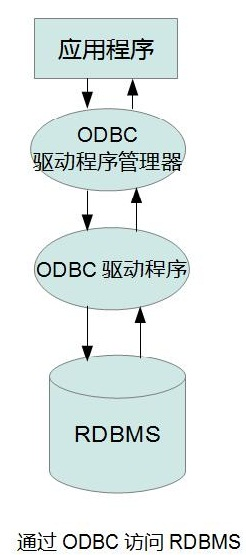
\includegraphics[height=5cm]{ODBC.jpg}
	\end{flushright}
\end{columns}	
\end{frame}
\subsection{PHP连接MySQL}
\begin{frame}{php连接mysql的4种方式}
	\begin{itemize}
		\item mysqli或mysql接口,用的较多
		\item pdo:{\tiny pdo为php访问数据库定义了一个轻量级的、一致性的接口。提供了一个数据访问抽象层,这样无论使用什么数据库,都可以通过一致的函数执行查询和获取数据。pdo本身并不能执行任何数据库操作,必须使用一个针对特定数据库的PDO驱动来访问数据库服务器。pdo\underline{\ }mysql,作为pdo针对mysql的驱动,新版php已经集成到php源码中,无需通过安装扩展来实现。}\footnote{\tiny 前三种连接方式的比较,官网手册上有个很好的说明:http://docs.php.net/manual/zh/mysqli.overview.php}
		\item ODBC:开放数据库连接,主要由微软主导,它建立了一组规范,并提供了一组针对所有语言访问数据库的标准API。
	\end{itemize}
\end{frame}
\begin{frame}
	\begin{center}
	{\LARGE THANK YOU !}
	\end{center}
%	\begin{block}{}
%	\begin{center}
%	{\small Proud to use \LaTeX\ and Beamer.}
%	\end{center}
%	\end{block}
\end{frame}
\end{CJK*}
\end{document} 